\chapter{Fazit}

Die Einsatzmöglichkeiten von Containern sind vielfältig. Sie erleichtern die Portierbarkeit von Anwendungen, sparen Platz und schonen die Ressourcen. Sie können Entwicklern dabei helfen, Fehlverhalten in ihrer Anwendung aufgrund unterschiedlicher Softwareversionen zu verhindern oder aber bei Bedarf in sehr kurzer Zeit beliebig viele Container zu einem Cluster von bestimmten Anwendungen oder Services zuzuschalten, um das System zu entlasten. Der einfachste Fall ist wohl eine einfache monolithische Webanwendung, die leicht transportiert und auf nahezu jedem System einfach ausgeführt werden kann. Jedoch laden Container dazu ein, eine Software in Microservices aufzuteilen, damit die jeweiligen Services möglichst isoliert von anderen Bestandteilen der Software arbeiten können und sich nicht etwa durch die Abhängigkeiten von den gleichen Bibliotheken in verschiedenen Versionen ausbremsen. Diese Kleinteiligkeit stellt Entwickler aber auch wieder vor neue Herausforderungen. Zwar sind die Container im einzelnen leicht portierbar und werden stabil in ihrer isolierten Umgebung laufen, aber sie müssen auch mit den anderen Services einer Anwendung verknüpft werden oder im entsprechenden Cluster einsortiert werden, um das volle Potential auszuschöpfen.\\

\noindent Docker-Swarm\footnote{https://www.docker.com/products/docker-swarm} ist ein internes Tool in der Docker-Engine das bei der Orchestrierung der Container hilft, also unter welchen Voraussetzungen welche Cluster hochskaliert werden, wann Container abgeschaltet werden oder dem Austausch von defekten Containern.
Aber auch für diesen Zweck gibt es bereits Cloud Computing Services, über die das Verwalten von Containern bzw. Container-Clustern vereinfacht wird. Was Infrastructure as a Service (IaaS) für virtuelle Server und Platform as a Service (PaaS) für fertige Laufzeitumgebungen ist, ist Container as a Service (CaaS) für Container. CaaS ist irgendwo zwischen IaaS und PaaS anzusiedeln, ähnelt aber vor allem IaaS, mit dem Unterschied, dass Container und nicht virtuelle Maschinen die vermieteten Ressourcen sind. Die CaaS Plattformen helfen dabei vor allem bei der Orchestrierung der Container. Bekannte Anbieter sind vor allem Amazon EC2 Container Service\footnote{https://aws.amazon.com/de/ecs/} und Google Kubernetes\footnote{https://kubernetes.io/}.\\

\noindent Zusammenfassend lässt sich sagen, dass das Prinzip von Containern zwar schon länger bekannt ist, aber erst seit einigen Jahren erfährt die Technologie vermehrt Beachtung, da durch Unternehmen wie Docker endlich eine vereinfachte Schnittstelle für Entwickler geschaffen wurde, um mit Containern zu arbeiten. Es gibt zwar noch einige kritische Stimmen, die vor allem Bedenken wegen der Sicherheit von Containern äußern, dennoch bergen sie vor allem viele Möglichkeiten für Entwickler ihre Anwendungen stabiler und flexibler zu gestalten.\\
% 
% \centering
% 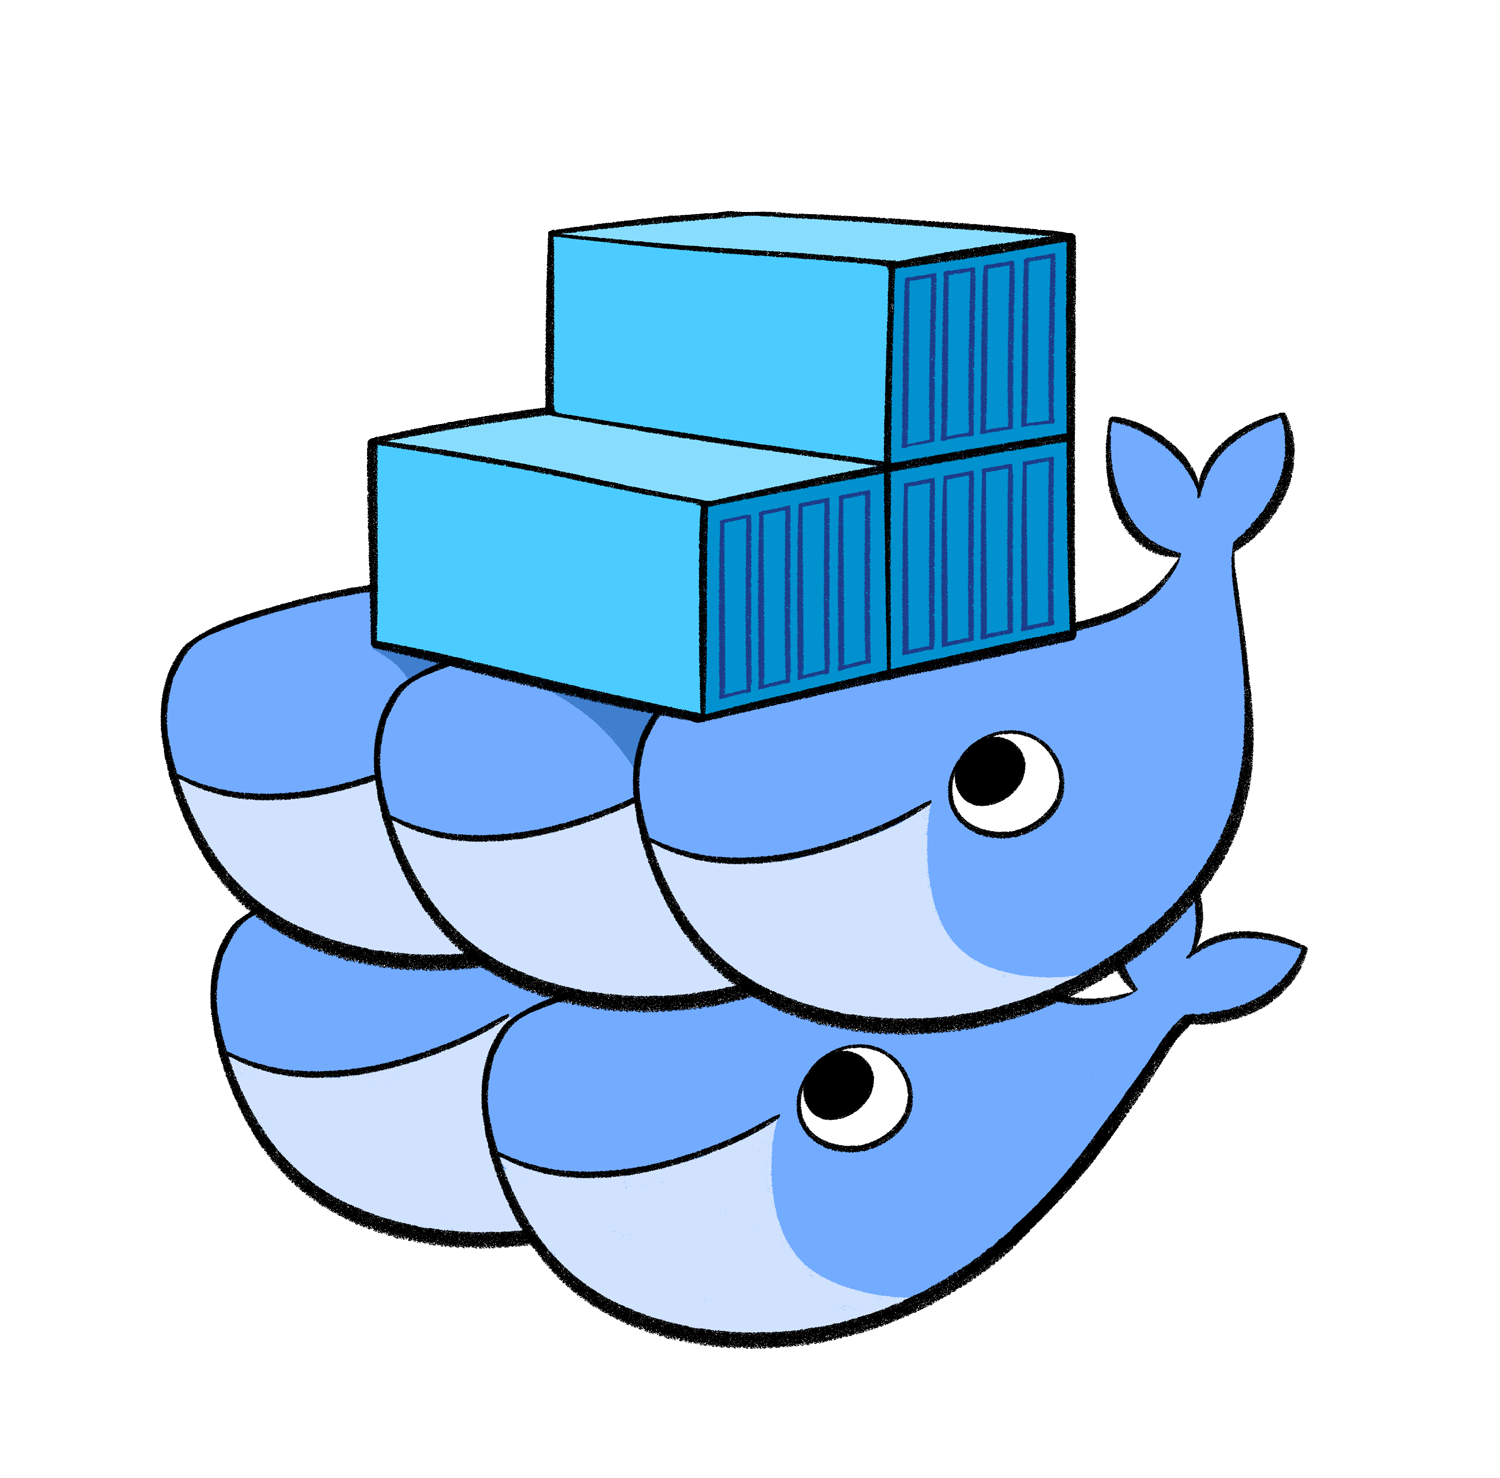
\includegraphics[width=0.5\textwidth]{images/14-docker-swarm-hero2.png}
